\documentclass[12pt]{article}
\usepackage[utf8]{inputenc}

\title{Specyfikacja implementacyjna}
\author{Patryk Zaniewski}
\date{11.11.2018}

\usepackage{natbib}
\usepackage{graphicx}
\usepackage{polski}

\begin{document}

\maketitle

\tableofcontents
\newpage

\section{Wstęp}
Problemem, który porusza program jest rynek wymiany walut. Pięciu spekulantów potrzebuje programu, który w prosty sposób pomoże im osiągnąć jak największy zysk. Oczekują oni, że dostarczony im program będzie realizował dwie funkcje. Pierwszą z nich jest wyznaczanie ścieżki wymiany walut. Dodatkowo, taka ścieżka musi być jak najbardziej dochodowa dla użytkownika. Drugą z funkcji jest możliwość wyznaczenia dowolnego arbitrażu walutowego na podstawie ilości pieniędzy przez nas posiadanych.

\section{Wykorzystane technologie i środowiska programistyczne}
Do napisania programu zostanie wykorzystany język Java w wersji 11. Program będzie realizowany w środowisku programistycznym Intellij Idea 2018 firmy JetBrains.


\section{Opis wykorzystanych algorytmów}
Program poza standardowymi algorytmami wczytania, walidacji oraz wypisania danych będzie zawierał szereg innych algorytmów. Odpowiedzialne one będą za właściwe przekazywanie kursów walut do struktury grafu, wyszukanie najkorzystniejszej ścieżki wymiany waluty wejściowej na wyjściową oraz za wyszukanie arbitrażu walutowego.
\newline\newline
Algorytm przekazywania i umieszczania danych w strukturze będzie opierał się na liście list. Każda z walut będzie posiadała własną listę sąsiadów z której będzie można odczytać do jakiej innej waluty wyjściowej możemy przewalutować aktualną walutę. Dodatkowo, graf będzie zawierał informacje o kursach między walutami oraz o opłatach ponoszonych przy wymianie.
\newline\newline
Algorytmem odpowiedzialnym za wyszukanie najkorzystniejszej ścieżki wymiany walut będzie algorytm Bellmana-Forda. Jednak dla jego poprawnego działania należy wszystkie koszty przewalutowań przedstawić w postaci: \textbf{1/koszt przewalutowania}. Sprawi to, że algorytm wyznaczy najkrótszą ścieżkę dla odwróconych liczb, a co za tym idzie największy mnożnik przewalutowania między walutą wejściową, a wyjściową.


 
\section{Diagram klas}
Na poniższym diagramie \emph{Rysunek 1} zostały zobrazowane zależności między klasami w programie. Każda z klas zostanie szczegółowo opisana w kolejnym punkcie. W diagramie zostały pominięte metody get() i set(), jako nie wpływające znacząco na logikę aplikacji - na diagramie mogłyby przysłonić bardziej istotne elementy.

\begin{figure}[h!]
\centering
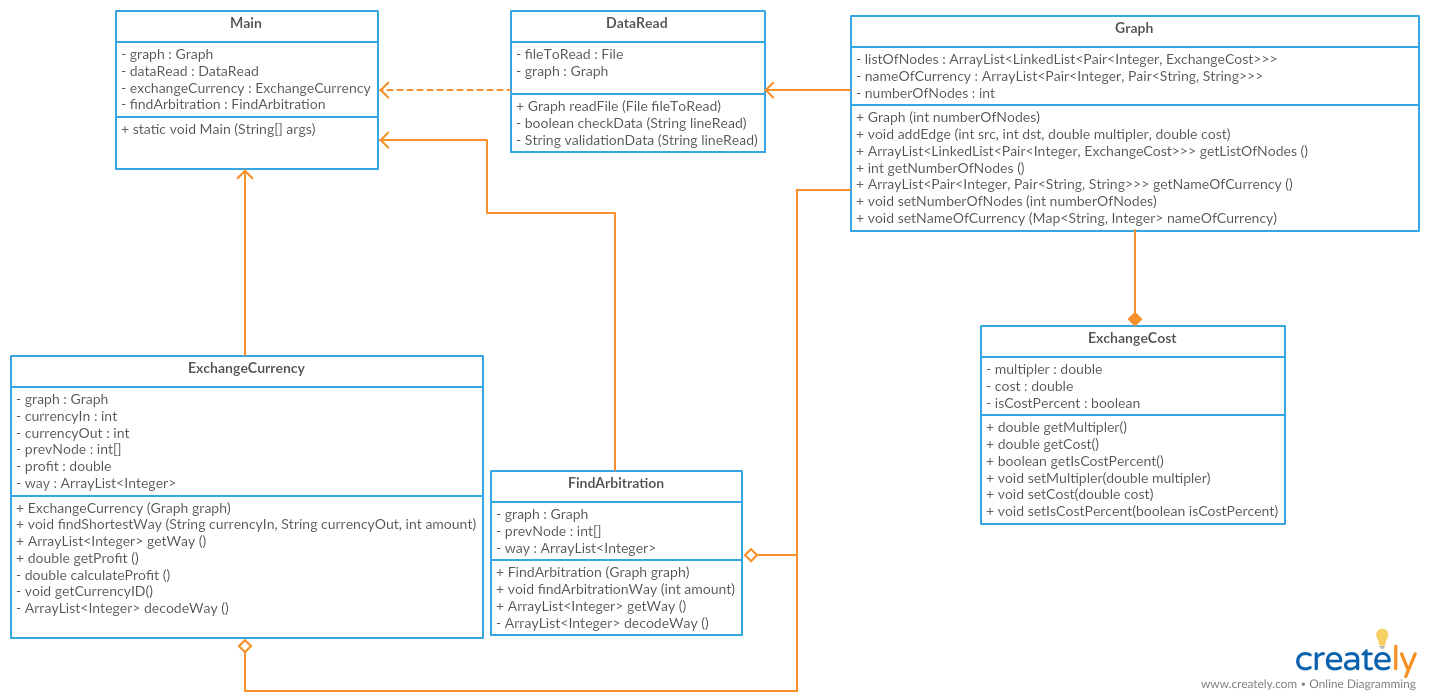
\includegraphics[scale=0.5]{diagram}
\caption{diagram klas}
\label{fig:diagram}
\end{figure}

\section{Opis klas i metod}

\section{Spis zaimportowanych pakietów}
W programie zostaną zaimportowane i użyte pakiety wymienione poniżej. 
\begin{enumerate}
    \item java.lang
    \item java.util
    \item java.io
    
\end{enumerate}

\section{Testy jednostkowe}
Testy jednostkowe generowane będą za pomocą narzędzia JUnit za pomocą którego otrzymamy możliwość sprawdzenia poszczególnych metod w klasach.
Przykładowe testy:
\end{document}
